\documentclass{jot} 

\usepackage{amssymb}
\setcounter{tocdepth}{3}
\usepackage{graphicx} 
\usepackage{verbatim}
\usepackage{listings}
\usepackage{multicol}
\usepackage{textcomp}
\usepackage{courier}
\usepackage{wrapfig}
\usepackage{longtable}
\usepackage[T1]{fontenc}
\usepackage{lmodern}
\usepackage{shortvrb}
\usepackage{url}

\usepackage[utf8]{inputenc}
%\usepackage[T1]{fontenc}
\usepackage[english]{babel}
\usepackage{microtype}
\usepackage{tabularx,booktabs}
\usepackage{xspace}
%\usepackage{textcomp}
%\usepackage{listings}
% \usepackage{graphicx}
%\graphicspath{{./figures/}}


\lstdefinelanguage{EOL}{
morekeywords={delete,import,for,while,in,and,or,self,operation,return,def,var,throw,if,new,else,transaction,abort,break,continue,assert,assertError,not},
sensitive=true,
morecomment=[l]{//},
%morecomment=[s]{/*}{*/},
morestring=[b]",
showstringspaces=false
}
\lstdefinelanguage{EVL}
{morekeywords={for, import, context, typeOf, kindOf, high, medium, low, constraint, critique, check, do, message, title, fix, not, guard, in, and, or, operation, return, var, def, if, new, else, delete},
sensitive=true,
morecomment=[l]{//},
%morecomment=[s]{/*}{*/},
morestring=[b]',
showstringspaces=false,
}

\renewcommand\dblfloatpagefraction{.99}
\renewcommand\dbltopfraction{.99}
\renewcommand\floatpagefraction{.99}
\renewcommand\topfraction{.99}
\renewcommand\bottomfraction{.99}
\renewcommand\textfraction{.01}
%\addtolength{\belowcaptionskip}{-8mm}
%\addtolength{\abovecaptionskip}{-5mm}
%\setlength{\intextsep}{1mm}

\newcommand\parambegin{\rmfamily\textlangle\itshape}
\newcommand\paramend{\upshape\textrangle}
\newcommand\parameter[1]{{\parambegin#1\paramend}}
\newcommand\code[1]{\texttt{#1}}
\let\file\code
\newcommand\jotcls{\file{jot.cls}\xspace}
\newcommand\JOT{\caps{JOT}\xspace}


\lstset{
	language=[LaTeX]TeX,
	escapeinside={_}{_},
	escapebegin={\rmfamily\textlangle\itshape},
	escapeend={\upshape\textrangle},
	gobble=4
}
\lstMakeShortInline[ % typeset sequences |like this| as code
escapeinside={_}{_},
escapebegin=\parambegin,
escapeend=\paramend
]|

%
%\lstset{ 
%  upquote=true,
%	captionpos=b,
%	breaklines=true,
%	xleftmargin=0pt,
%	basicstyle=\ttfamily\scriptsize,
%	flexiblecolumns=true,
%	%numbers=left,
%	nolol=true,
%	tabsize=2,
%	escapechar=\$
%  showstringspaces=false,
%} 


%\newcommand{\keywords}[1]{\par\addvspace\baselineskip
%\noindent\keywordname\enspace\ignorespaces#1}

\title{An Approach for Efficient Querying of Large Relational Datasets with OCL-based Languages}
\runningtitle{Efficient Querying of Relational Dataset with OCL-Based Languages}

\author[affiliation=dlut]
{Ran Wei}
{   is an associate professor at the Dalian University of Technology, China.
	Contact him at \email{r.wei@live.co.uk}.}

\author[affiliation=uoy]
{Konstantinos Barmpis}
{   is a researcher of the Department of Computer Science at the University of York, United Kingdom. 
	Contact him at \email{konstantinos.barmpis@york.ac.uk}.}

\author[affiliation=uoy]
{Dimitrios Kolovos}
{   is a professor of the Department of Computer Science at the University of York, United Kingdom.
	Contact him at \email{dimitris.kolovos@york.ac.uk}.}

\affiliation{dlut}{Dalian University of Technology, China\\ \url{http://www.dlut.edu.cn}}
\affiliation{uoy}{University of York, United Kingdom\\ \url{http://www.york.ac.uk}}

\runningauthor{R. Wei, K. Barmpis and D. Kolovos.}
\jotdetails{
	volume=0,
	articleno=0,
	year=2010,
}


\begin{document}
\begin{abstract}
Relational database management systems are used to store and manage large sets of data, subsets of which can be of interest in the context of Model Driven Engineering processes. 

To enable seamless integration of information stored in relational databases in an MDE process, the technical and conceptual gap between the two technical spaces needs to be bridged. 
In this paper we investigate the challenges involved in querying large relational datasets using an imperative OCL-based model management language (EOL) through running examples, and we propose solutions for some of these challenges.
\end{abstract}
\maketitle


%\keywords{Metamodelling, Domain, Modelling, MDE}

\section{Introduction}

Information that can potentially be of interest in the context of a Model Driven Engineering (MDE) process is often located within non-model artefacts such as spreadsheets, XML documents and relational databases. 
As such, model management languages and tools would arguably benefit from extending their scope beyond the narrow boundaries of 3-level metamodelling architectures such as EMF and MOF for MDE.

In previous work, we have demonstrated how OCL-based model management (e.g. model validation, model-to-text and model-to-model transformation) languages of the Epsilon platform \cite{EpsilonICECCS} can be used to interact with plain XML documents~\cite{EpsilonXML} and spreadsheets~\cite{EpsilonSpreadsheets}. 
In this work we investigate the challenges involved in using such languages to query large relational datasets and extract abstract models that can be then used (e.g. analysed, validated, transformed) in the context of MDE processes.
In particular, we identify the challenges imposed by the size of such datasets and the conceptual gap between the organisation of relational databases and the object-oriented syntax of OCL-based languages, and we propose some solutions.

The rest of the paper is organised as follows. 
In Section \ref{sec:approach} we present a running example that involves querying a real-world large relational dataset and extracting an EMF model from it using an OCL-based imperative transformation language, we identify the performance challenges involved in doing so, and propose a run-time query translation approach that addresses some of these challenges. 
In Section \ref{sec:background}, we review previous work on using OCL to query relational datasets and compare our approach to it, and in Section \ref{sec:conclusions} we conclude the paper and provide directions for further work.
\section{Querying Large Relational Datasets: Challenges and Solutions}
\label{sec:approach}

The Epsilon Object Language \cite{EOL} is an OCL-based imperative model query and transformation language. EOL is the core language of the Epsilon platform and underpins a number of task-specific languages for model management tasks including model validation, model-to-model and model-to-text transformation. As such, by adding support for querying relational datasets to EOL, this capability is automatically propagated to all task-specific languages of the platform. While the discussion in the rest of the paper focuses on EOL, in principle the discussion and solutions proposed are also relevant to a wide range of OCL-based model management languages such as QVTo, ATL and Kermeta.

To experiment with querying relational datasets with EOL, we selected a large real-world publicly-available dataset from the US Bureau of Transportation Statistics\footnote{\url{http://www.transtats.bts.gov/DL_SelectFields.asp?Table_ID=236&DB_Short_Name=On-Time}} that records all domestic flights in the US in January 2013. The dataset consists of one table (Flight) with 223 columns and 506,312 rows and is 221MB when persisted in MySQL. Each row of the table records the details of a domestic flight during that month, including the short codes of its origin and destination airports, the flight's departure and arrival time etc. An excerpt of the Flight table appears in Figure \ref{fig:database}. 

Our aim in this running example is to transform this dataset into an EMF model that conforms to the metamodel of Figure \ref{fig:atms} and which captures the incoming and outgoing routes for each airport as well as the volume of traffic on these routes, so that we can then further process the EMF model to discover interesting facts about the structure of the US airport network.

\begin{figure}[ht]
\centering
\begin{minipage}[b]{0.47\linewidth}
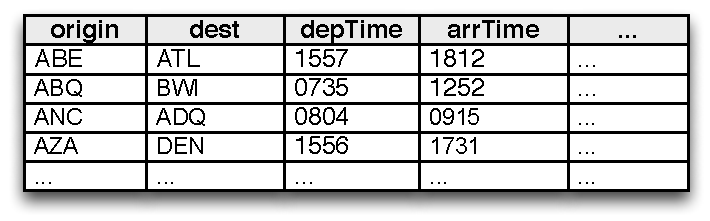
\includegraphics[width=2.3in]{images/database.pdf}
\caption{Excerpt of the Flight table}
\label{fig:database}
\end{minipage}
\quad
\begin{minipage}[b]{0.47\linewidth}
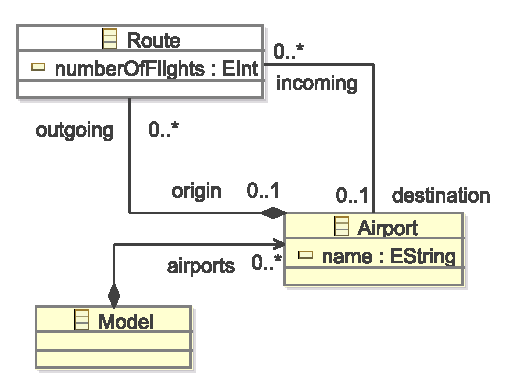
\includegraphics[width=2.3in]{images/atms.pdf}
\caption{Simple ATM System Metamodel}
\label{fig:atms}
\end{minipage}
\end{figure}

%\begin{figure}
% \centering
%		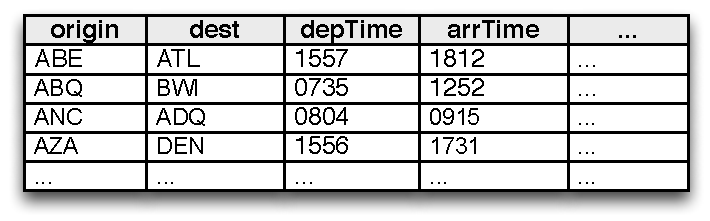
\includegraphics[width=0.6\textwidth]{images/database.pdf}
%	\caption{Excerpt from the Flight table}
%	\label{fig:database}
%\end{figure}
%
%\begin{figure}
% \centering
%		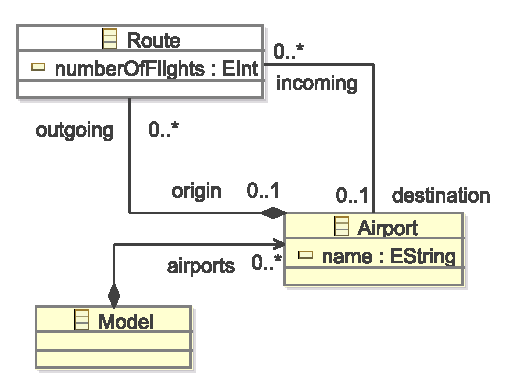
\includegraphics[width=0.7\textwidth]{images/atms.pdf}
%	\caption{Simple ATM System Metamodel}
%	\label{fig:atms}
%\end{figure}

\subsection{Finding the number of airports in the network}

A reasonable OCL-like expression\footnote{EOL does away with the ocl- prefixes (e.g. oclAsSet()) and the $\rightarrow$ OCL operator and uses . instead for all property/method calls.} that can be used to retrieve the number of all distinct airports\footnote{We assume that there are no airports with only incoming or outgoing flights and as such, looking into one of \emph{origin}, \emph{dest} should suffice.} in the Flight table would be:

\begin{lstlisting}
Flight.allInstances.origin.asSet().size()
\end{lstlisting}

When such an expression is evaluated against an in-memory model (e.g. an EMF model) the EOL execution engine performs the following steps:
\begin{enumerate}
  \item It inspects the model and computes a collection of all model elements of type Flight;
  \item It iterates through the contents of the collection computed in step 1 and collects the values of their \emph{origin} properties in a new collection;
  \item It removes all duplicates from the collection computed in step 2;
  \item It computes the size of the collection computed in step 3.
\end{enumerate}

To evaluate the same expression against the relational database discussed above, we can assume that each table in the database is a type and each row in the table is a model element that is an instance of that type. Under these assumptions, the following issues emerge:
\begin{enumerate}
  \item To compute the \emph{Flight.allInstances} collection, the engine needs to execute the following SQL query: \emph{select * from Flight}. Due to the size of the Flight table, the returned result-set cannot fit in a reasonable amount of heap space (we experimented with up to 1GB), and as such it needs to be streamed from the database to the engine instead. Streamed result-sets demonstrate the following challenges:
  \subitem They support forward-only iteration;
  \subitem To calculate the size of a streamed result-set it needs to be exhaustively iterated (in which case it becomes unusable as only forward iteration is permitted);
  \subitem Each database connection cannot support more than one streamed result-sets at a time.
  \item Iterating through all rows of the Flight table through a streamed result set and collecting the values of the \emph{origin} column of each row is particularly inefficient given that the same result can be achieved at a fraction of the time using the following SQL statement: \emph{select origin from Flight};
  \item Eliminating duplicates by iterating the collection computed in step 2 is also inefficient as the same result can be achieved using the following -- more efficient -- SQL statement: \emph{select distinct origin from Flight};
  \item Finally, calculating the size of a streamed result-set is not trivial without invalidating the result-set itself. By contrast, this could be computed in one step using the following SQL statement: \emph{select count(distinct origin) from Flight}.
\end{enumerate}

\subsection{Finding adjunct airports}

Assuming that we have computed a set containing the short codes of all airports in the table, the next task is to find for each airport, which other airports are directly connected to it, and then compute the volume of traffic between each pair of adjunct airports. An imperative EOL program that can be used to achieve this follows:

\begin{lstlisting}[language=EOL, numbers=left]
var origins = Flight.allInstances.origin.asSet();
for (origin in origins) {
	var destinations = Flight.allInstances.dest.asSet();
	for (destination in destinations) {
		var numberOfFlights = Flight.allInstances.
			select(f|f.origin = origin and f.dest = destination).
				size();
	}
}
\end{lstlisting}

The following observations can be made for the program above:

\begin{itemize}
  \item Although the \emph{destinations} result-set computed in line 3 does not change, it needs to be re-computed for every nested iteration as the result of the computation is streamed, and therefore only permits forward navigation;
  \item Unless care is taken to evaluate the right-hand side expressions in lines 1 and 3 using different database connections, the program will fail (as discussed above, each MySQL connection only permits at most one streamed result-set at a time);
  \item Iterating through all the rows of the Flight table in the \emph{select(\ldots)} method in lines 5-7 is inefficient, particularly as the same result can be computed using the following SQL statement \emph{select count(*) from Flight where origin=? and destination=?} (where \emph{?} should be replaced every time with the appropriate origin/destination values).
\end{itemize}

\subsection{Runtime SQL Query Generation}

%By now, readers should be convinced that querying relational datasets using OCL-like languages is a really bad idea in terms of performance, and that SQL is a more natural and performant language to query such data. 

In this section we argue that while the naive way of evaluating OCL-like queries on relational datasets can dramatically degrade performance (as shown in the previous section), there are certain runtime optimisations that the execution engine can perform to significantly reduce the execution time and memory footprint of some types of queries.

After applying such optimisations, the following EOL transformation, can transform the complete dataset (DB) in question to an EMF-based model (ATMS) that conforms to the metamodel of Figure \ref{fig:atms} in less than 45 seconds on average hardware\footnote{CPU: 2.66 GHz Intel Core 2 Duo, RAM: 8 GB DDR3.}. A visualisation of an excerpt of the extracted model appears in Figure \ref{fig:model}.

The functionality of the transformation is outlined below:
\begin{itemize}
  \item In line 1 it creates a new instance of the \emph{Model} EClass in the ATMS EMF (target) model;
  \item In line 2 it computes a set of all origin airports in the Flight table;
  \item In line 4 it iterates through the set of strings computed in line 2;
  \item In line 5 it invokes the \emph{airportForName} method defined in lines 21-30 which returns an instance of the \emph{Airport} EClass in the target model with a matching name;
  \item In lines 6-7 it computes a set of adjunct airports to the origin airport;
  \item In lines 10-12 for each adjunct airport (destination), it computes the number of flights between the two airports;
  \item In lines 13-16 it creates a new instance of the \emph{Route} EClass in the target model and populates its origin, destination and numberOfFlights properties.
  \item The \emph{airportForName()} method in lines 21-30 is responsible for preventing the creation of airports with duplicate names in the target model.
\end{itemize}

\begin{lstlisting}[language=EOL, label=lst:eol, caption=EOL transformation, numbers=left]
var m : new ATMS!Model;
var origins = DB!Flight.allInstances.origin.asSet();

for (origin in origins) {
	var originAirport = airportForName(origin);
	var destinations = DB!Flight.allInstances.
		select(f|f.origin = origin).dest.asSet();
	
	for (destination in destinations) {
		var numberOfFlights = DB!Flight.allInstances.
			select(f|f.origin = origin and f.dest = destination)
				.size();
		var route = new ATMS!Route;
		route.origin = originAirport;
		route.destination = airportForName(destination);
		route.numberOfFlights = numberOfFlights.asInteger();
	}
	
}

operation airportForName(name : String) {
	var airport = ATMS!Airport.allInstances.
		selectOne(a|a.name = name);
		
	if (airport.isUndefined()) {
		airport = new ATMS!Airport;
		airport.name = name;
		m.airports.add(airport);
	}
	return airport;
}
\end{lstlisting}

\begin{figure}
 \centering
		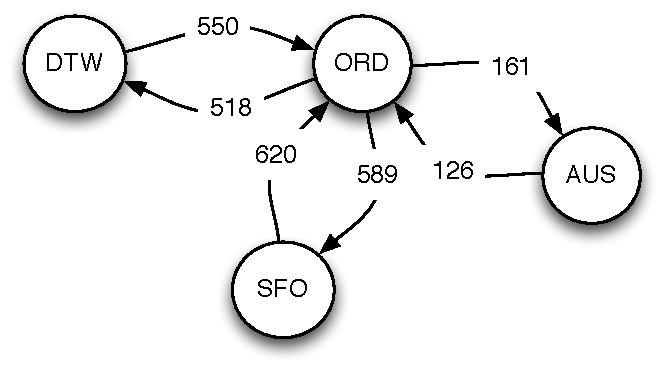
\includegraphics[width=0.5\textwidth]{images/model.pdf}
	\caption{Visualisation of an excerpt of the model extracted using the transformation in Listing \ref{lst:eol}}
	\label{fig:model}
\end{figure}

To achieve an acceptable level of performance, we have extended the EOL execution engine to use streamed \emph{lazy collections} and a runtime OCL to SQL query translation strategy for certain types of OCL expressions when the latter are evaluated against relational datasets. Each lazy collection acts as a wrapper for an SQL query generated at runtime and only starts streaming data from the database if/when it needs to be iterated. This prevents unnecessary database queries and enables multi-step query translation at runtime. An example of the query translation process is illustrated in Figure \ref{fig:query} which calculates the average delay of flights flying from JFK to LAX on Sundays. In particular, the following OCL expressions are rewritten as SQL queries.

\begin{description}

\item\textbf{.allInstances} Retrieving all the rows of a table in the database returns a streamed lazy collection (\emph{ResultSetList}) that is backed by a \emph{select * from <table>} SQL expression. For example, \emph{Flight.allInstances} is translated to \emph{select * from Flight}.

\item\textbf{.select(<iterator>|<condition>)} \emph{ResultSetList} overrides the built-in OCL select operation, translates the EOL condition to an SQL expression, and returns a new \emph{ResultSetList} constrained by the latter. For example, \emph{Flight. allInstances.select(f|f.origin = "JFK" and f.dayOfWeek=1)} is translated into \emph{select * from Flight where origin = ? and dayOfWeek = ?} (the values of the parameters -- i.e. JFK and 1 -- are kept separately and are only used if the query needs to be executed). The condition can contain references to the columns of the table, arithmetic, and logical operators at arbitrary levels of nesting. The \emph{exists()}, \emph{forAll()} and \emph{reject()} OCL operations behave similarly.

\item\textbf{.collect(<iterator>|<expression>)} \emph{ResultSetList} overrides the built-in OCL collect() operation to return a streamed lazy collection of primitive values (\emph{PrimitiveValuesList}). For example, \emph{Flight.all.collect(f|f.dest + "-" + f.origin)} is translated to \emph{select origin + "-" + dest from Flight}. In the spirit of OCL, retrieving properties of collections is a short-hand notation for collect(). For example, \emph{Flight.allInstances.dest} is shorthand for \emph{Flight.allInstances. collect(f|f.dest)}.

\item\textbf{.size()} Calls to the size() method of a \emph{ResultSetList}/\emph{PrimitiveValuesList} are interpreted as \emph{count} SQL queries. For example \emph{Flight.allInstances.size()} is translated to \emph{select count(*) from Flight}.

\item\textbf{asSet()} Calls to asSet() method of a \emph{PrimitiveValuesList} return a new \emph{PrimitiveValuesList} backed by a \emph{distinct} SQL query. For example, \emph{Flight.allInstances. dest.asSet()} returns a new \emph{PrimitiveValuesList} backed by the following SQL query: \emph{select distinct(dest) from Flight}. 

\end{description}

\begin{figure}
 \centering
		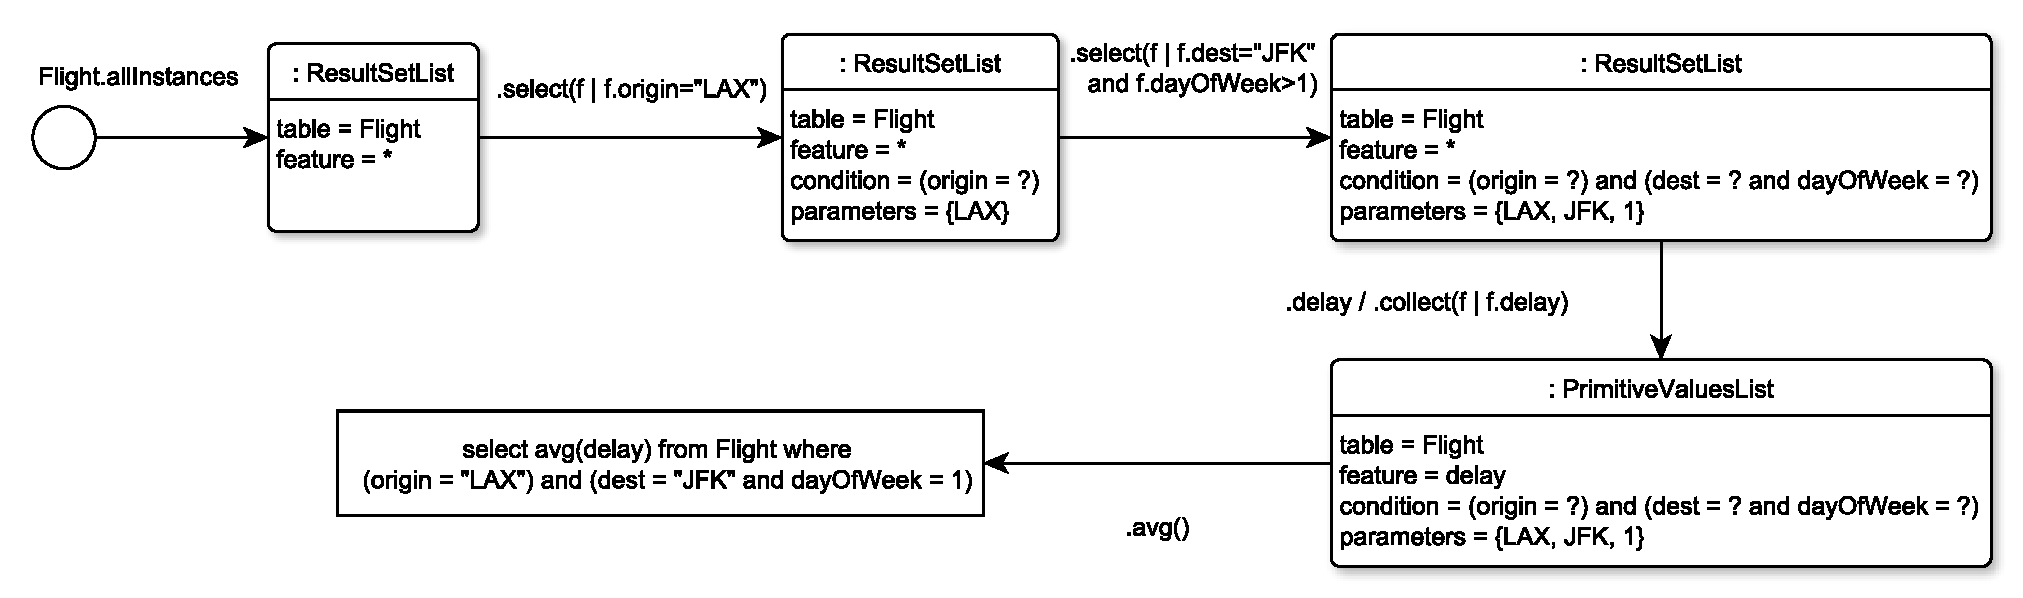
\includegraphics[width=\textwidth]{images/query.pdf}
	\caption{Multi-step SQL query generation process}
	\label{fig:query}
\end{figure}

Streamed lazy collections also provide a \emph{fetch()} method that executes their underpinning query and returns a complete in-memory result-set which is navigable in both directions. This is useful for small result-sets where the overhead of maintaining the entire result-set is memory is preferable to the performance overhead of streaming. To address the limitation of one streamed result-set per connection, we are using a pool of connections for streamed result-sets: each streamed result-set requests a connection from the pool when it needs to be computed and returns it back to the pool when it has been fully iterated.

%\begin{itemize}
%  \item Evaluating an \emph{.allInstances} expression on a type X originating from a relational dataset (e.g. \emph{DB!Flight.allInstances}) returns a streamed lazy collection (\emph{ResultSetList}) that is backed by a \emph{select * from X} SQL query, which is not executed until the collection starts being iterated;
%  \item Evaluating a \emph{.size()} expression on a streamed\emph{ResultSetList} executes an SQL count query (i.e. \emph{select count(*) from X}) instead of iterating through the contents of the list;
%  \item Evaluating a property call expression on a streamed \emph{ResultSetList} (e.g. \emph{DB!Flight.allInstances.dest}) returns a streamed lazy collection  (\emph{PrimitiveValuesList}) backed by a \emph{select property from X} SQL query;
%  \item Evaluating an \emph{.asSet()} expression on a streamed \emph{PrimitiveValuesList}, returns a new streamed \emph{PrimitiveValuesList} backed by a \emph{select distinct property from X} SQL query;
%  \item Evaluating a \emph{.select(x|x.a = b)} expression on a streamed \emph{ResultSetList}, returns a new streamed \emph{ResultSetList} backed by a \emph{select * from X where a = ?}. Nested \emph{select()} expressions are interpreted as and'ed SQL conditions.
%\end{itemize}


%As discussed above, 
%
%\begin{lstlisting}
%context Flight {
%	constraint OriginAndDestMustDiffer {
%		check : self.origin <> self.dest
%		message: "Flight " + self.id + " has the same origin and destination airports"
%	}
%}
%\end{lstlisting}

%\subsection{Extracted Facts}
%
%Some interesting facts that may or may not end up in the paper due to space restrictions.
%
%\begin{itemize}
%  \item There are 306 airports in the dataset. Of these, 68 are connected directly to only 1 other airport;
%  \item After running Dijkstra's shortest path algorithm for all airports in the model, it was found that the most distant pair of airports in the network are Leihigh Valley International Airport (ABE) and Wiley Post-Will Rogers Memorial Airport (BRW). A passenger wishing to travel between the two would need to change 4 flights (ABE$\rightarrow$DTW$\rightarrow$SEA$\rightarrow$FAI$\rightarrow$BRW);
%  \item The Atlanta International Airport (ATL) is the busiest airport in terms of the number of flights that go through it (67,717), followed by ORD, DFW, DEN, LAX and IAH;
%  \item ATL is also the best-connected airport with direct flights to 148 airports in the country;
%  \item ORD and DEN are the best-connected airports in terms of the number of airports that passengers can reach with direct or 1-stop flights (301), followed by ATL, IAH and DFW (294), and DTW (292);
%  \item \textgreater50\% of all the flights go through the 18 busiest airports and \textgreater90\% of all flights go through the 91 busiest airports.
%\end{itemize}
\section{Related Work}
\label{sec:background}
%The following articles/web resources appear to be relevant: \cite{Berrabah2007}, \cite{Demuth2001}

Several researchers have proposed solutions for translating OCL to SQL. For example, in \cite{Berrabah2007}, the authors demonstrate an approach for generating event-condition-action (ECA) rules comprising SQL triggers and procedures from OCL constraints attached to a UML class diagram, when the latter is translated into a relational schema. In \cite{Demuth2001}, the authors propose using OCL-derived views in relational databases designed using UML, to check the integrity of the persisted data. In this work each OCL constraint is translated into a view in the relational database that contains reports of integrity violations. Such violations can be handled using different strategies including rolling back the offending transaction, triggering a data reconciliation action, or simply reporting the violation to application users. This approach has been implemented in the context of the OCL2SQL prototype\footnote{\url{http://dresden-ocl.sourceforge.net/usage/ocl22sql/}}. A similar approach is proposed by the authors of \cite{Marder2009}. In \cite{Heidenreich2007}, the authors propose a framework for translating OCL invariants into multiple query languages including SQL and XQuery using model-to-text transformations.

All the approaches above propose compile-time translation of OCL to SQL. By contrast, our approach proposes run-time generation and lazy evaluation of SQL statements. While compile-time translation is feasible for side-effect free OCL constraints that are evaluated against a homogeneous target (e.g. a relational database), for use-cases that involve querying and modifying models conforming to different technologies (e.g. a relational database and an EMF model), this approach is not applicable. Another novelty of the approach proposed in this paper is that it does not require a UML model that specifies the schema of the database, and as such, it can be used on existing databases that have not been developed in a UML-driven manner.
\section{Conclusions and Further Work}
\label{sec:conclusions}

In this paper we have argued that it is important for model management languages to extend their scope beyond the narrow boundaries of 3-level metamodelling architectures such as MOF and EMF. In this direction, we have experimented with  using an OCL-based imperative transformation language to query data stored in relational databases. We have reported on the identified challenges and proposed an approach for improving the performance of some types of queries using run-time query translation.

In future iterations of this work, we plan to investigate the extent to which compile-time static analysis and query rewriting can deliver additional benefits in terms of performance. An obvious target is to use static analysis to limit the number of columns returned by queries by excluding any columns that are never accessed in the model management program, but additional optimisations are also envisioned. We also plan to investigate supporting queries spanning more than one tables by exploiting foreign keys.

\backmatter

\nocite{*}
\bibliographystyle{alphaurl}
\bibliography{reference}
\abouttheauthors

\begin{acknowledgments}
	This research was part supported by the EPSRC, through the Large-Scale Complex IT Systems project (EP/F001096/1) and by the EU, through the Automated Measurement and Analysis of Open Source Software (OSSMETER) FP7 STREP project (318736).
\end{acknowledgments}

\end{document}